\documentclass[tikz,border=8pt]{standalone}
\usepackage{amsmath,amssymb}
\usetikzlibrary{arrows.meta,positioning}

\begin{document}
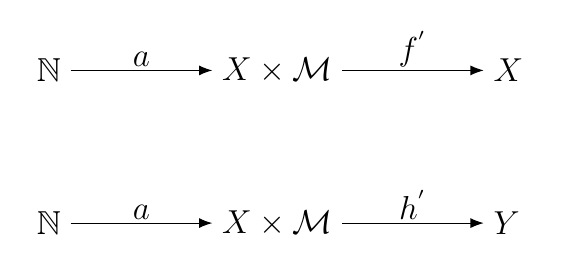
\begin{tikzpicture}[
  >=Latex,
  node distance=18mm,
  every node/.style={font=\large},
  lab/.style={midway, fill=white, inner sep=1.2pt}
]

% Nodes
\node (N1) {$\mathbb{N}$};
\node (XM1) [right=of N1] {$X \times \mathcal{M}$};
\node (X1)  [right=of XM1] {$X$};

\node (N2)  [below=14mm of N1] {$\mathbb{N}$};
\node (XM2) [right=of N2] {$X \times \mathcal{M}$};
\node (Y2)  [right=of XM2] {$Y$};

% Arrows + labels
\draw[->] (N1) -- (XM1) node[lab, above] {$a$};
\draw[->] (XM1) -- (X1) node[lab, above] {$f^{'}$};

\draw[->] (N2) -- (XM2) node[lab, above] {$a$};
\draw[->] (XM2) -- (Y2) node[lab, above] {$h^{'}$};

\end{tikzpicture}
\end{document}
